%%% Template originaly created by Karol Kozioł (mail@karol-koziol.net) and modified for ShareLaTeX use

\documentclass[a4paper,11.5pt]{article}
\usepackage{hyperref}
\usepackage{float}
\hypersetup{colorlinks,breaklinks,
            urlcolor=[rgb]{0,0.5,0.5},
            linkcolor=[rgb]{0,0.5,0.5}}
\usepackage[T1]{fontenc}
\usepackage[utf8]{inputenc}
\usepackage{graphicx}
\usepackage{xcolor}
\linespread{1.1}
\renewcommand\familydefault{\sfdefault}
\usepackage{tgheros}
\usepackage[defaultmono]{droidmono}
\usepackage{amsmath,amssymb,amsthm,textcomp}
\usepackage{enumerate}
\usepackage{multicol}
\usepackage{tikz}

\usepackage{geometry}
\geometry{total={210mm,297mm},
left=1.4in,right=1.4in,%
bindingoffset=0mm, top=20mm,bottom=20mm}

\newcommand{\linia}{\rule{\linewidth}{0.5pt}}

% custom theorems if needed
\newtheoremstyle{mytheor}
    {1ex}{1ex}{\normalfont}{0pt}{\scshape}{.}{1ex}
    {{\thmname{#1 }}{\thmnumber{#2}}{\thmnote{ (#3)}}}

\theoremstyle{mytheor}
\newtheorem{defi}{Definition}

% my own titles
\makeatletter
\renewcommand{\maketitle}{
\begin{center}
\vspace{2ex}
{\huge \textsc{\@title}}
\vspace{1ex}
\\
\linia\\
\@author \hfill \@date
\vspace{4ex}
\end{center}
}
\makeatother
%%%

% custom footers and headers
\usepackage{fancyhdr}
\pagestyle{fancy}
\lhead{}
\chead{}
\rhead{}
\lfoot{Ray Tracer}
\cfoot{}
\rfoot{Page \thepage}
\renewcommand{\headrulewidth}{0pt}
\renewcommand{\footrulewidth}{0pt}
%

% code listing settings
\usepackage{listings}
\lstset{
    language=C++,
    basicstyle=\fontsize{11}{11}\selectfont\ttfamily,
    aboveskip={1.0\baselineskip},
    belowskip={1.0\baselineskip},
    columns=fixed,
    extendedchars=true,
    breaklines=true,
    %tabsize=4,
    prebreak=\raisebox{0ex}[0ex][0ex]{\ensuremath{\hookleftarrow}},
    frame=lines,
    showtabs=false,
    showspaces=false,
    showstringspaces=false,
    keywordstyle=\color[rgb]{0.8,0,0},
    commentstyle=\color[rgb]{0.026,0.112,0.095},
    stringstyle=\color[rgb]{0.627,0.126,0.941},
    escapeinside={\%*}{*)}
}

%%%----------%%%----------%%%----------%%%----------%%%

\begin{document}

\title{Computer Graphics - Ray Tracer}

\author{Prisca Aeby}

\date{06/05/2015}

\maketitle

\section{The Camera Model}
\subsection{The Standard Camera Model}
The class I wrote for the camera model has been inspired by \href{http://web.cse.ohio-state.edu/~parent/classes/681/Lectures/08.RTgeometryHO.pdf}{this lecture} from the Ohio State University. The view plane is calculated in function of the field of view of the camera and the given width and height resolutions. The idea is to position the view plane at the point where the camera is looking and to calculate the bottom left point and the vectors to be incremented to render the entire image. The code below shows how those parameters are calculated in function of the field of view:
\begin{lstlisting}
halfWidth= std::abs(tan(fieldOfView/2));
float aspectRatio = heightRes / widthRes;
halfHeight = aspectRatio * halfWidth;
pixelWidth = 2 * halfWidth * planeDistance / widthRes;
pixelHeight = 2 * halfHeight * planeDistance / heightRes;
downLeft = lookAt - v*(halfHeight) - u*(halfWidth);
\end{lstlisting}
The multi-sample anti-aliasing is done by randomly choosing inside each pixel a number of samples and to take the average of all the sample colors. The colors are calculated in the \texttt{World::traceRay(Ray r, int depth)} function. The code below is showing how it is implemented:

\begin{lstlisting}
Vector3D xIncVector = u*2*halfWidth / widthRes;
Vector3D xAliasing = xIncVector / samples;
Vector3D yIncVector = v*2*halfHeight / (heightRes);
Vector3D yAliasing = yIncVector / samples;
for (int r = 0; r < heightRes; r++){
  for (int p = 0; p < samples; p++){
    for (int q = 0; q < samples; q++) {
      point = downLeft + xIncVector*c + yIncVector*r + xAliasing*(rand()%(int)samples) + yAliasing*(rand()%(int)samples);
      ray.o = point;
      ray.d = point - eyePos;
      ray.d.normalize();
      color = color + w->traceRay(ray, 0);
    }
  }
  color = color / (samples*samples);
  w->displayPixel(r, c, color);
}
\end{lstlisting}
Once a color is calculated it is saved in the \texttt{World} class with the call to the \texttt{displayPixel} function. My images are saved in the BMP file format but first I store all the values in a three dimensional matrices keeping the final red, green and blue values for each pixel. 
\begin{figure}[H]
\centering
\makebox[\textwidth]{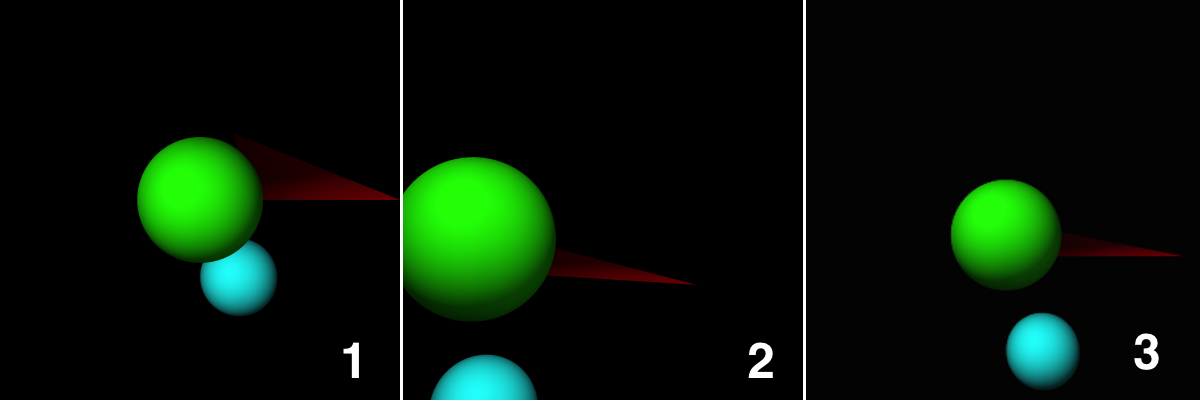
\includegraphics[width=\textwidth]{camera.png}}
\end{figure}
The first image is generated from the point (0,0,0) looking at the point (0,0,20) with a field of view of 166 degrees. The second image's camera has the same field of view but it is placed at the point (10,20,0) and is looking closer at the object. The third camera is positioned at the same place that the second one but I enlarged the field of view to 175 degrees.

\subsection{Adding Depth Of Field Effects}
I added a \texttt{DOFCamera} class which takes as arguments the same ones as the standard \texttt{Camera} and in addition a focal length and a lens radius parameters. The idea to generate depth of field effects is to mime the behaviour of a camera. The primary rays aren't sent only from one fixed point but from a lens with a given radius. You can see below an image explaining the parameters I used in my code and I will explain in detail afterwards what I have done. 
\begin{figure}[H]
\centering
\makebox[\textwidth]{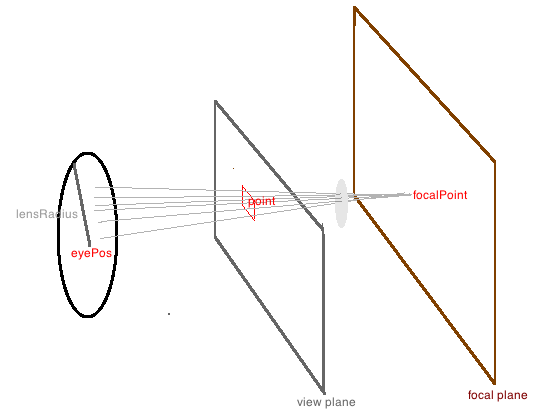
\includegraphics[width=250px]{dof.png}}
\end{figure}
The goal is to send for each pixel primary rays from several points around the \texttt{eyePos} in the direction of the focal point. the focal point is obtained by multiplying the point on the view plane by the factor \texttt{focalLength/viewPlaneDistance}. As you can see on the schema above, if the object is on the focal plane it will give the same result for each ray sent around the eye position. But if the object lies behing or between the view plane and the focal plane like the grey circle, the hit points will be different for one pixel and therefore the color will vary. The code given below is the modification added to the standard camera model. I give the code generating a random point around the eye position too. 
\clearpage
\begin{lstlisting}
//the sample pixel on the viewplane that is taken randomly from the square of one pixel
point = downLeft + xIncVector*c + yIncVector*r + xAliasing*(rand()%(int)samples) + yAliasing*(rand()%(int)samples);
lensPoint = randomLensPoint();
//the point on the focal plane:
Point focalPoint = point*(focalLength/planeDistance);
//the direction is the point on the focal plane minus the point on the lens
ray.d = focalPoint-lensPoint;
ray.o = lensPoint;
color = color + w->traceRay(ray, 0);
\end{lstlisting}
\begin{lstlisting}
Point DOFCamera::randomLensPoint(){
  double r, phi; // polar coordinates
  Point sp;
  r =  (rand()) / (RAND_MAX/lensRadius);
  phi = (rand()) / (RAND_MAX/(2.0*3.141592653));
  sp.x = eyePos.x +  r * cos(phi);
  sp.y = eyePos.y + r * sin(phi);
  return sp;
}

\end{lstlisting}
\begin{figure}[H]
\centering
\makebox[\textwidth]{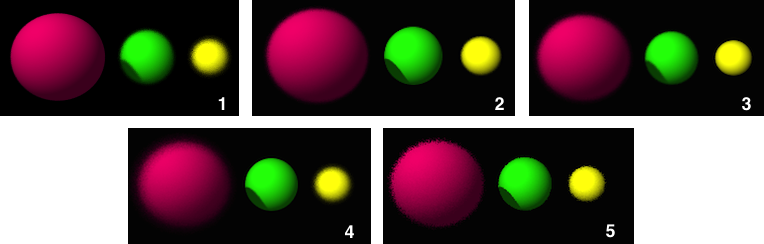
\includegraphics[width=550px]{depth.png}}
\end{figure}
The picture above shows different settings of the camera. The three spheres have the same radius but the first one is placed at 50 along the w axis, the second one at 80 and the third one at 120. The first three images have a lens radius of 2 and there are 100 samples per each pixel. The parameter changing is the focal length. On the first one it is set at 50, then at 80 and finally at 120. Only the sphere positioned at the focal length will appear clearly. The fourth image has the same settings as the second image but the lens radius is this time of 6. This is why the objects not placed on the focal plane are appearing more blury. The points generated from the eye position are in a bigger range. The fifth image has the same parameter as the second image but I reduced the number of samples to 25. 
\section{Transforming The Objects}
When we want to find if a transformed object is hit by a ray the technique is to first apply the inverse transformation to the ray and then check the intersection between this new ray and the untransformed object. In order to keep the transformation information, each \texttt{Object} has three transformation matrices (translation, rotation, scaling) which are modified every time we apply a transformation to an object. If an object has been transformed it affects not only its hit position but the normal where it has been hit too. You can find below the function iterating through the objects and checking the closest intersection:
\begin{lstlisting}
for (std::vector<Object*>::iterator it = objects.begin(); it != objects.end(); ++it){
  transformedMatrix = (*((*(*it)->scalingMatrix->inverse())*((*it)->rotateMatrix->inverse())))*((*it)->translateMatrix->inverse());
  transformedRay.o = *transformedMatrix*(&r.o);
  transformedRay.d = (*((*(*it)->scalingMatrix->inverse())*((*it)->rotateMatrix->inverse())))*(&r.d);
  hitInfo = (*it)->hit(transformedRay);
  if((hitInfo.t != -1) and (hitInfo.t < tmin)){
    tmin = hitInfo.t;
    hitNearest = hitInfo;
    hitNearest.intersectPoint = *((*((*(*it)->translateMatrix)*((*it)->rotateMatrix)))*((*it)->scalingMatrix))*&hitInfo.intersectPoint;
    hitNearest.normal = (*((*(*it)->rotateMatrix)*((*it)->scalingMatrix->inverse())))*(&hitInfo.normal);
    hitNearest.normal.normalize();
    nearestObject = *it;
  }
}
return nearestObject->material->shade(&hitNearest, this, &r);
\end{lstlisting}
As you can see in the code above, when an object has been hit it returns a \texttt{hitResult} object which contains the distance between the hit point and the plane, the normal where the object has been hit and the intersection point. As we will see in the light part we need the normal to calculate the intensity of the color. If an object has been transformed, we need to transform its normal too. It is achieved by multiplying the untransformed normal by the rotation matrix and the inverse of the scaling matrix. 
\begin{figure}[H]
\centering
\makebox[\textwidth]{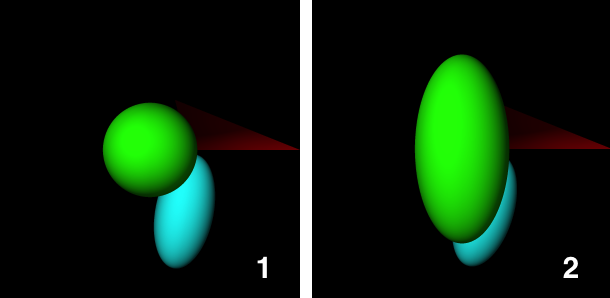
\includegraphics[width=300px]{transform.png}}
\end{figure} 
The first image is generated by applying sphere2->rotate\_z(0.2)
then sphere2->scale(1,2,1) and finally sphere2->translate(10.0,20.0,0.0). The second image uses the stack transformation functionality: it adds the objects to a vector std::vector<Object*> scaleObj and then calls the \texttt{World} function w->scale(1.0,2.0,1.0, scaleObj). In the class \texttt{World} there is a function for each transformation which takes a vector of objects and then iterates through this list and call the correspondant \texttt{Object} transformation function.
\section{Primitives}
All the primitives herit from the class \texttt{Object}. The attributes/functions of this class are the transform matrices/functions that we already mentioned and the \texttt{hit(Ray ray)} function that returns a \texttt{hitResult} object. I took the functions calculating the intersections in the \textit{Ray Tracing from the Ground Up} book. Each \texttt{Object} has a reference to its \texttt{Material}. We will see in the next section how this class is implemented. 
\begin{itemize}
\item \textbf{Triangle:} triangles are defined by their three points. Its constructor looks like this: \texttt{Triangle(Point* a, Point* b, Point* c, bool smoothTriangle)}. In the builder of a \texttt{Triangle} we calculate its normal \texttt{(Vector3D(*p2-*p1))$\wedge$(Vector3D(*p3-*p1))}. When a hit ocurs we return in the \texttt{hitResult} this normal if it is not a smooth triangle. In the other case, we return the interpolated normal of the three normals definining the triangle: \texttt{(Vector3D(*p2-*p1))$\wedge$(Vector3D(*p3-*p1))}.
\item \textbf{Plane:} a plane is defined by a point and a normal. The normal returned in the hit is always the same.
\item\textbf{ Sphere: }a \texttt{Sphere} is defined by its center and its radius. I use the scaling transformation option to generate ellipsoids. 
\end{itemize}
\section{Object Material}
Each \texttt{Object} has a pointer to a \texttt{Material} and each \texttt{Material} has a \texttt{RGBColor} attribute and a \texttt{shade(hitResult* hitInfo, World* w, Ray* r)} function which returns a \texttt{RGBColor} in function of the lights added to the \texttt{World}. I implemented two types of material, the \texttt{Matte} one and the \texttt{Specular} one.
\subsection{Matte Material}
This \texttt{Material} has a diffuse attribute and a color. You can see below its \texttt{shade} function: 
\begin{lstlisting}
Matte::shade(hitResult* hitInfo, World* w, Ray* r) {
  RGBColor L = color * w->ambientLight;
  int num_lights = w->lights.size();
  for (int j = 0; j < num_lights; j++) {
    Vector3D lightDirection = w->lights[j]->get_direction(hitInfo->intersectPoint);
    double lightOnSurface = hitInfo->normal * (-lightDirection);
    if (lightOnSurface > 0.0){
      if(! (w->lights[j]->inShadow(new Ray(hitInfo->intersectPoint, -lightDirection), w))){
        L += (color * 0.3183098*kd) * w->lights[j]->radiance * lightOnSurface;
        }
      }
    }
  return (L);
}
\end{lstlisting}
First of all, the \texttt{World} gives an ambient color and even if there is no light added to the \texttt{World} we can see the color of the objects in function of the intensity of this ambient light. Then for each \texttt{Light} of the \texttt{World} we check if the dot product between the negative direction of the \texttt{Light} and normal of the object where it has been hit is positive. In this case, the light is lighting the object. There is a test for checking if it is actually reaching the object or not but we will see it in detail in the shadow part. The more the light direction and the normal are parallel to each other the bigger the \texttt{lightOnSurface} parameter will be and therefore the brighter the color will be. Each \texttt{Light} has a radiance that will affect the brightness of the object too.

\subsection{Specular Material}
This \texttt{Material} is a bit more elaborated than a basic \texttt{Material}. In fact, in addition to its diffuse coefficient it has a reflection coefficient and a specular exponent that reflects the \texttt{Light} in a different way. When a \texttt{Light} hit this \texttt{Specular} material it has to send a new \texttt{Ray} to the entire \texttt{World} reflecting the light which hit it. This \href{http://paulbourke.net/geometry/reflected/}{simple geometry} helped me to calculate the direction of the reflected ray. You can see below the \texttt{shade} function:
\begin{lstlisting}
RGBColor Specular::shade(hitResult* hitInfo, World* w, Ray* r) {
  RGBColor L = phong(hitInfo, w, r);
  Vector3D viewDirection = -r->d;
  double i = hitInfo->normal * viewDirection;
  Vector3D reflectedDir = r->d + hitInfo->normal * i * 2.0;
  Ray reflected_ray = Ray(hitInfo->intersectPoint, reflectedDir);
  reflected_ray.reflexions = r->reflexions + 1;
  L += w->traceRay(reflected_ray, reflected_ray.reflexions)
  return (L);
}
\end{lstlisting} 
First we calculate the \texttt{Phong} color generated by all the lights in the \texttt{World}. In the \texttt{Phong} distribution the object appears shiny if the direction from which the ray is sent and the reflected ray of the light coincide. The more parallel they are to each other the brighter the color will be. Then we calculate the reflected ray and we have to trace it again through the \texttt{World}. The code for the \text{Phong} illumination is given below. If there is no Phong brightness, it returns the color in the same way as the \texttt{Matte} material.
\begin{lstlisting}
RGBColor Specular::phong(hitResult* hitInfo, World* w, Ray* r){
  Vector3D viewDirection = -r->d;
  RGBColor L = color*w->ambientLight;
  int num_lights = w->lights.size();
  for (int j = 0; j < num_lights; j++){
    Vector3D lightDirection = w->lights[j]->get_direction(hitInfo->intersectPoint);
    double lightOnSurface = hitInfo->normal * lightDirection;
    if(lightOnSurface > 0.0){
      if(! (w->lights[j]->inShadow(new Ray(hitInfo->intersectPoint, -lightDirection), w))){
        Vector3D mirror = Vector3D(-lightDirection + hitInfo->normal * lightOnSurface * 2.0);
        double phongSurface = mirror * viewDirection;
        RGBColor spec;
        if(phongSurface > 0.0){
          spec = RGBColor(1,1,1) * kr * pow(phongSurface, e);
        }
        L +=  (color*kd*0.318309 + spec)*w->lights[j]->radiance)*lightOnSurface;
      }
    }
  }
  return L;
}
\end{lstlisting}
You can see below a picture of the pink ball and the green ball having two different Specular materials and the other objects having normal Matte material. The green sphere has a diffuse coefficient of 0.4, a reflective coefficient of 0.8 and a specular exponent of 5. The pink sphere has a diffuse coefficient of 0.8, a reflective coefficient of 0.3 and a specular exponent of 10. You can see the light of the green ball reflected on the right side of the pink ball. 
\begin{figure}[H]
\centering
\makebox[\textwidth]{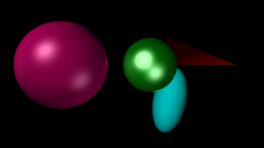
\includegraphics[width=200px]{material.png}}
\end{figure} 
I just want to mention here a problem I encountered first when I was generating the images. In fact, the parts of the spheres supposed to be bright were suddenly black like you can see in the picture above.
\begin{figure}[H]
\centering
\makebox[\textwidth]{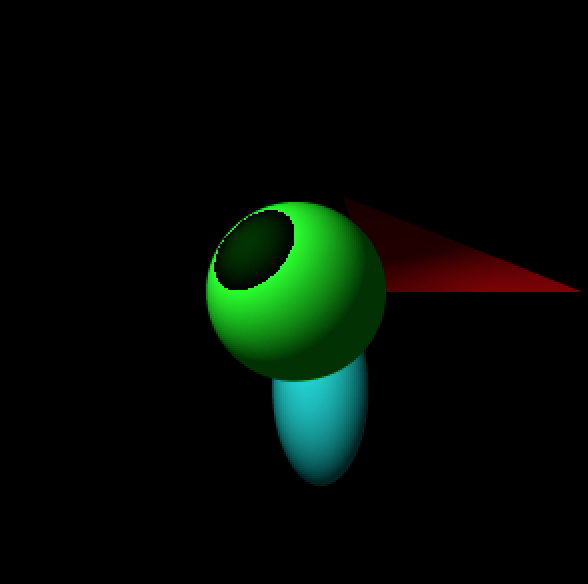
\includegraphics[width=100px]{black.png}}
\end{figure}
It was due to the fact that the RGB color values were out of range because they were larger than one due to the phong effect. I adjusted the function \texttt{displayPixel} in the class \texttt{World} to readjust the colors out of range. You can find the code below:
\begin{lstlisting}
void World::displayPixel(int r, int c, RGBColor color){
  double max_value = max(color.r, max(color.g, color.b));
  RGBColor adjustedColor;
  if(max_value > 1.0){
    adjustedColor = color/max_value;
  }
  else{
    adjustedColor = color;
  }
  image[r][c][0] = adjustedColor.r;
  image[r][c][1] = adjustedColor.g;
  image[r][c][2] = adjustedColor.b;
}
\end{lstlisting} 
\section{Lighting}
\subsection{Point Lights}
I have defined one class for the \texttt{Light}. Its constructer looks like this \texttt{light(Vector3D* dir, Point* position, double radiance, bool dir)}. The boolean indicates if it is a point light with a direction or not. We already saw in the \texttt{Material} class that for calculating the brightness of a point we iterate through all the lights and accumulate the effects of each light for one pixel. For calculating the impact of one light we have to take two things into account. The first thing that affects the intensity is the vector between the light position and the hit point. It has been taken into account in the shade function from each material. The function get\_direction of the class light returns this vector. But if the light has a direction we have to adapt its radiance too. The radiance will vary in function of the distance between the point light and the object and it will be influenced by the distance between the normal at the hit point and the direction of the light. If the light has no direction we simply return the normalised vector between the point hit and and the position of the light and the intensity remains constant. You can find below the code returning the direction and adapting the radiance:
\begin{lstlisting}
Vector3D light::get\_direction(Point p, Normal normal){
  if(dir){
  double distance = (normal.distance(direction));
  radiance = radianceTemp/(p.d_squared(&position)*((distance*distance)+distance));
  }
  return (Vector3D(position-p)).hat();
}
\end{lstlisting}
You can see on the image below the effect of the point light. I decided to show three exactly identical spheres with just the color changing to show the intensity varying with the distance. 
\begin{figure}[H]
\centering
\makebox[\textwidth]{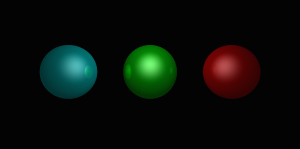
\includegraphics[width=150px]{pointlight.png}}
\end{figure}
\subsection{Shadows}
In the \texttt{Material shade} function we take the effect of a light on the object only if the light is not stopped by an other object. The idea is to send back a shadow ray which has the opposit direction to the light and see if it hits an object between the position of the source of the light and the point hit. This check is done by the call to the \texttt{light::inShadow(Ray* shadowRay, World* w)} function. The code of this function is given below:
\begin{lstlisting}
bool light::inShadow(Ray* shadowRay, World* w){
  double d = position.distance(&shadowRay->o);
  Matrix* transformedMatrix;
  Ray transformedRay;
  hitResult hitInfo;
  for (std::vector<Object*>::iterator it = w->objects.begin(); it != w->objects.end(); ++it){
    transformedMatrix = (*((*(*it)->scaleMatrix->inverse())*((*it)->rotateMatrix->inverse())))*((*it)->translateMatrix->inverse());
    transformedRay.o = *transformedMatrix*(&shadowRay->o);
    transformedRay.d = (*((*(*it)->scaleMatrix->inverse())*((*it)->rotateMatrix->inverse())))*(&shadowRay->d);
    hitInfo = (*it)->hit(transformedRay);
    if(hitInfo.t > 0.0001 and (hitInfo.t < d)){
      return true;
    }
  return false;
}
\end{lstlisting}
What it does is that it first calculates the distance between the light and the point that has been hit. Then it iterates through all the objects and check if one of them is between the light source and the point. As soon as it finds an object it returns true. You can notice that we take into account the objects that have been transformed.   

\begin{figure}[H]
\centering
\makebox[\textwidth]{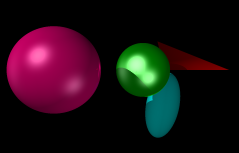
\includegraphics[width=280px]{shadow.png}}
\end{figure} 
Here is an example when the shadows are activated. The pink sphere stopped the light source to the green sphere but there is still an other light affecting the green pshere. The blue ellipsoid has the shadow of the green and pink spheres and the red triangle has the shadow of the green sphere.
\end{document}